\documentstyle[11pt,dectab,theapa,icann92,psfig,icanedit,wrapfig]{article}
\def\x#1#2{\mbox{$#1\times#2$}}
\def\X#1{\mbox{$\times#1$}}
\citepunct{[}{\&}{\&}{ }{; }{, }{]}{}{.}
\citelabels{, ed.}{, eds.}{Vol.}{No.}{edition}%
{p.}{pp.}{chap}{Tech report}
\psfigurepath{../postscript/}

\begin{document}
\bibliographystyle{theapa}

\title{The Speed and Slips of Mental Arithmetic}
\author{Richard Dallaway (richardd@cogs.susx.ac.uk)}
\firstpage{1369}
\showwherepublished
\maketitle

\begin{abstract}
The literature on arithmetic memory offers a number of theories for how we
succeed and fail in recalling basic facts (such as $\x34=12$).
\citeA{mcclmode} have noted that these theories lack detailed
implementations, and as such are difficult to appraise.  This paper
presents a connectionist model of memory for multiplication facts. The
system's behaviour is compared to the error patterns and reaction times
(RTs) of adults reported by \citeA{harlasso} and \citeA{millcogn}.
\end{abstract}

\subsection*{Introduction}



Adults exhibit well documented patterns of behaviour when recalling
multiplication facts. RTs generally increase across the multiplication
tables, but this ``problem-size effect'' has plenty of exceptions (see
fig.~\ref{rt01}). Tie problems (\x22, \x33 etc.)\  are
recalled relatively quickly. In addition to this \citeA{camp85} found that
adults make errors at the rate of 7.65 per cent, and of those errors 92.6
per cent fall into the following categories:
%%%%%%%%%%%%%
{\em Operand errors}, for which the
erroneous product for the problem \x a b is a member of the $a$ or $b$
multiplication table (e.g., $\x65=45$);
%%%%%%%%%%%%%
{\em Close operand
errors}, where the erroneous product is an operand error and also close in
magnitude to the correct product. That is, for the problem \x a b, the
error will often be correct for the problem $a\pm2\times b$ or $a\times
b\pm2$ (e.g., $\x65=40$);
%%%%%%%%%%%%%
{\em Frequent products} are
the five products 12, 16, 18, 24 and 36;
%%%%%%%%%%%%%
{\em Table errors},
where the erroneous product is the correct answer to some problem, but does
not share any digits with the presented problem (e.g., \x65=16);
%%%%%%%%%%%%%
{\em Operation errors}, where the error to \x a b is correct
for $a+b$.
%%%%%%%%%%%%%
The remaining 7.4 per cent of {\em non-table errors} were not correct
products for any of the problems \x00 to \x99.

Five or six years of classroom drill does ensure that multiplication facts
are ready to hand, but it does not ensure perfect recall. The problem is to
produce a model which has correctly learnt the tables, yet can make slips
when recalling answers. This aspect is missing from the other PDP model of
mental arithmetic \cite{andestud}, which is based around the BSB algorithm.
As presented the BSB model
lacks the ability to correctly answer some problems,
or fails to respond at all.

Given the observations on the types of erroneous responses, and the RT for
correct responses, what assumptions must be made? The model
presented here suggests that the initial skew in the frequency and order of
presentation of multiplication fact \cite[p.~118]{camprole} is
one of the important factors.

\subsection*{Architecture}

A multilayered network
is trained on all the problems \x00 through \x99 in a random
order using backpropagation. The two digits that comprise a problem are
coarse encoded on the two%
\begin{wrapfigure}[21]{r}{7.1cm}\fboxsep=2pt
\noindent\fbox{\psfig{file=x01rt.ps,width=6.9cm,clip=}}
\caption{Plot of mean correct RT per multiplication table collapsed over
operand order for: median RT of 42 adults
\protect\cite[app.~D]{harlasso};
median RT (adjusted for naming time) of 6 adults
\protect\cite[table~A1]{millcogn};
mean RT for 20 networks trained on skewed frequencies; and, the same 20
networks after continued training on uniform frequencies (both networks
equally scaled).}
\label{rt01}\end{wrapfigure}
sets of 10 input units (representing the
digits 0--9).  For tie problems, an additional tie bit is set to 1.
Activation flows through a hidden layer of 12 units, to the output layer.
There is one output unit per product, plus a ``don't know'' unit.

During training, the presentation frequency of each pattern is skewed
according to the problem frequencies reported by \citeA{siegmult}. Although
problems with small products do occur more frequently in textbooks, there
is no reason to believe this skew continues into adulthood \cite[p.
328]{mcclmode}.  Hence, after 35~000 epochs on skewed data (to a mean total
sum squared error, tss, of 0.07) the network is trained for a further
35~000 epochs with equal frequencies (reaching a mean tss of 0.002).  After
training both the ``skewed'' and ``equalized'' networks can correctly
recall all the patterns in the training set.

The ``cascade'' equations \cite[p.~153]{pdp3} are used to simulate the
spread of activation in the network.  Each unit's activity is allowed to
build up over time:
\def\net{\mbox{net}}
\[ \net_i(t) = k \sum\limits_j w_{ij} a_j(t) + (1-k)\ \net_i(t-1),\]
\noindent where: $k$ determines the rate with
which activation builds up (0.05); $w$ is the weight matrix; and $a_j(t)$
is the activation of unit $j$ at time $t$. The $\net_i$ is passed through
the logistic squashing function to produce the activation value, $a_j$, and
the response values are taken to be the normalized activation values
(outputs sum to 1.0). Fig.~\ref{act01plot} is a time plot of output
responses using the cascade equations.

\subsection*{Simulations}

At the start of cascade processing the initial state of the network is that
which results from processing an all-zeros input pattern (to give all
patterns a common starting point). The network is trained to activate the
``don't know'' unit for all-zeros input. For each problem a random
threshold is selected between 0.4 and 0.9. Processing continues until a
product unit exceeds this threshold. The RT (number of cascade steps) is
recorded for a correct response, and erroneous responses are classified
into the five categories itemized above. The network is presented with each
of the 100 problems 50 times, and the mean correct RT is recorded.  This is
repeated for 20 networks with different initial weights.



With a large threshold the correct product is reliably recalled, but
occasionally the threshold will be low enough to accept an incorrect
product. For example, ``12'' would be a close operand error for \x44 in
fig.~\ref{act01plot}. Presumably the mild time pressure of the experimental
situation results in subjects lowering their thresholds.


\subsection*{Results}
The mean RTs plotted in fig.~\ref{rt01} show some of the basic features of
the problem-size effect.  For the skewed networks the RT correlates
$r=0.22$ ($p=0.013$) with adult RT reported by \citeA{millcogn}. This
increases to $r=0.37$ ($p=0.000067$) for the equalized networks. Slightly
lower correlations were found to the \citeA{harlasso} RTs. Note that the
RTs have reduced and
flattened out for the equalized networks, which is
just what is expected after continued practice
\cite[p.~349]{camp85}. One
feature of the RT plot is the drop in RT for the nine times table. Children
in grades 3 to~5 respond faster to \X9 than \X8 problems \cite{camp85}, but
this levels out for adults.  The tie bit is required to ensure
that tie
problems are among the fastest. All tie problems were below the mean for
their table,%
\begin{wrapfigure}[32]{r}{7.1cm}\fboxsep=2pt
\noindent\fbox{\psfig{file=p4x4.ps,width=6.9cm,clip=}}
\caption{Response of the output units over 40 time steps for the problem
\x44.  Output units for products over 18 are not shown on this
graph.}
\label{act01plot}
\end{wrapfigure}
except for \x66. A comparison of error types is presented in
table~\ref{err01pc}.\begin{table*}
%\fbox{\vbox{\vspace{5mm}
\caption{Percentage breakdown of errors. Figures are mean values from
twenty different networks, and mean values from 42 adult subjects
\protect\cite[app.~B]{harlasso}. Adult scores other than
error frequency were recomputed from Harley's data.}
\begin{center}

\setdec 00.0
\def\notedag{\mbox{\raise 1mm\hbox{\footnotesize\dag}}}

\begin{tabular}{lccc}
\hline
&\multicolumn{2}{c}{Networks}&Adults\\
\cline{2-3} &Skewed&Equalized&\\
\hline
Operand errors          &\dec 93.56 &\dec 93.15 &\dec 86.20 \\
Close operand errors    &\dec 78.14 &\dec 74.12 &\dec 76.74 \\
Frequent product errors\notedag &\dec 22.56 &\dec 20.14 &\dec 26.99 \\
Table errors            &\dec 6.43  &\dec 6.85  &\dec 13.80 \\
%high operation due to 0xN=N
%Operation error         &\dec 2.21  &\dec 1.81  &\dec 13.72 \\
Error frequency         &\dec 10.64 &\dec 15.58 &\dec 6.3 \\
\hline
\multicolumn{4}{l}{\dag Percentage of operand errors.}
\end{tabular}

\end{center}
\label{err01pc}
%}}
\end{table*}


A correlation was found between problem error rate and correct RT.
\citeA[p.~110]{camprole} reports a correlation of 0.93 for adults.  For the
skewed and equalized networks $r=0.74$ and $r=0.76$ respectively.  It is
not obvious that any model would necessarily predict that slower problems
produce more errors.

Subjects sometimes respond with a number that is not a correct
product for any of the problems \x22 to \x99 (e.g., $\x23=5$). As the
network can only produce \x00 to \x99 products as output, it cannot produce
these non-table errors.  \citeA{camp85} report that only 7.4 per cent of
errors are of this kind.

\subsection*{Analysis and discussion}

Presentation frequency, product frequency, initial weight values, and input
encoding are all involved in determining the weights, which in turn
determines the RT.  Further assumptions suggested by other theories
\cite{siegmult,camp85} were not required. In particular there was no need
to explicitly train erroneous products, nor incorporate explicit global
magnitude information, or between-product connections.

The presentation frequency peaks slightly for the five times table. This
may be the reason behind the speed of the fives, but earlier simulations
using a linearly skewed
frequency curve also produced the characteristic dip.  It
should be noted that all the products in the five times table are unique in
the sense that they do not occur outside the context of 5 (unlike 12 which
occurs twice as often as any 5 product). The ``12'' output unit will need
to respond to two different encodings, where as all 5 output units will
only respond to one encoding (the networks learn the same encoding for
\x{a}{b} and \x{b}{a}).

It is often stated that \x0N problems are answered by rules. The
evidence cited to support this notion is mostly from the relative RTs of
zero problems \cite{millcogn,staznetw}. From the model's RTs it appears
that a rule is not required: zero problems have strong associations and are
quick to be recalled. However, this means that zero also occurs as an error
in unrealistic situations ($\x38=0$).  Harley's \citeyear{harlasso} results
show subjects producing errors of the form $\x0N=N$, which is rarely
observed in this model.  Also, \citeA{sokocogn} produce evidence to support
the notion of a rule: one of their brain damaged patients showed errors of
$\x0N=N$ on almost all \x0N problems, and then suddenly improved to almost
perfect performance on these problems [p.~358]. These points indicate that
it is the error performance, and not the RT, that suggests the special
status (though not necessarily a rule) for \x0N.

\subsection*{Acknowledgements} Funded by the SERC in conjunction with
Integral Solutions Ltd. Thanks to Harry Barrow and David Young. Simulations
were performed using a modified version of the \citeA{pdp3} {\em bp}
program, and POPLOG POP-11.
\bibliography{bib}
\end{document}
